\documentclass{beamer}
\title{The Sudoku Project}
\subtitle{WEEK 7: 05/09/2021 to 11/09/2021}
\author[Ishika | Yashvi]{Ishika De and Yashvi Donga}
\date{August - September 2021}

\usetheme{Madrid}

\begin{document}
\begin{frame}
     \titlepage
\end{frame}
\begin{frame}
     \frametitle{Agenda}
     \begin{itemize}
          \item Brief Overview
          \item Current Status
          \item Toolchain
          \item Difficulties
          \item Learnings
     \end{itemize}
\end{frame}

\begin{frame}
     \frametitle{Brief Overview}
     The goal of this project is to investigate a variety of algorithms (backtracking, brute force, stochastic search, depth first search) that are capable of solving
standard Sudoku puzzles, of ranging difficulties, in order to learn more about Sudoku
solving techniques.\newline

     We also wanted to create the sudoku solver using OpenCV that will read a puzzle from an image and solve it. We plan on using OpenCV for multiple programming languages.
\end{frame}

\begin{frame}
     \frametitle{Current Status}   
     \begin{itemize}
		  \item Implemented Backtracking and Brute Force Algorithm to solve a Sudoku in C++, Java and Python.
		  \item Tested 100 Sudokus of different difficulties for Backtracking and Brute Force Algorithm in C++, Java and Python.
		  \item Generated a graph to compare the algorithms and languages with respect to time taken.
		  \item Tried implementing Stochastic Simulated Annealing Algorithm in Python. (Not working for all cases) 
		  \item Tried implementing Crook's Algorithm in Python. (Not working for all cases)
	 \end{itemize}
\end{frame}

\begin{frame}
     \frametitle{Current Status}   
     \begin{itemize}
		  \item RESULTS
		  \begin{figure}
		  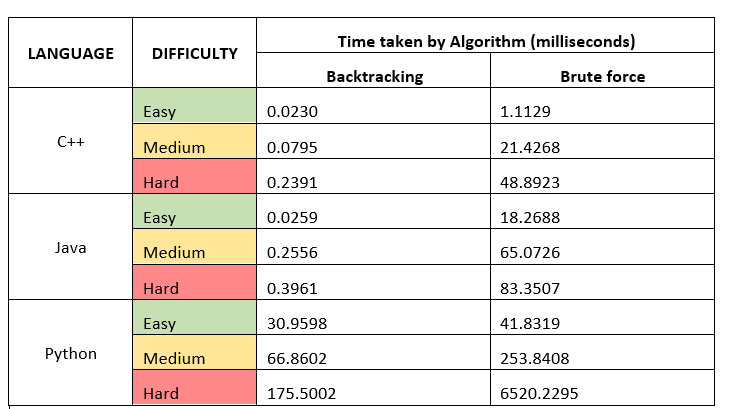
\includegraphics[width=0.9\textwidth]{./week7_img/sudoku_result_table.png}
		  \caption{Results: Average time taken to solve a sudoku (Tested 100 puzzles).}
		  \centering
		  \end{figure}
	 \end{itemize}
\end{frame}

\begin{frame}
     \frametitle{Current Status}   
		  \begin{figure}
		  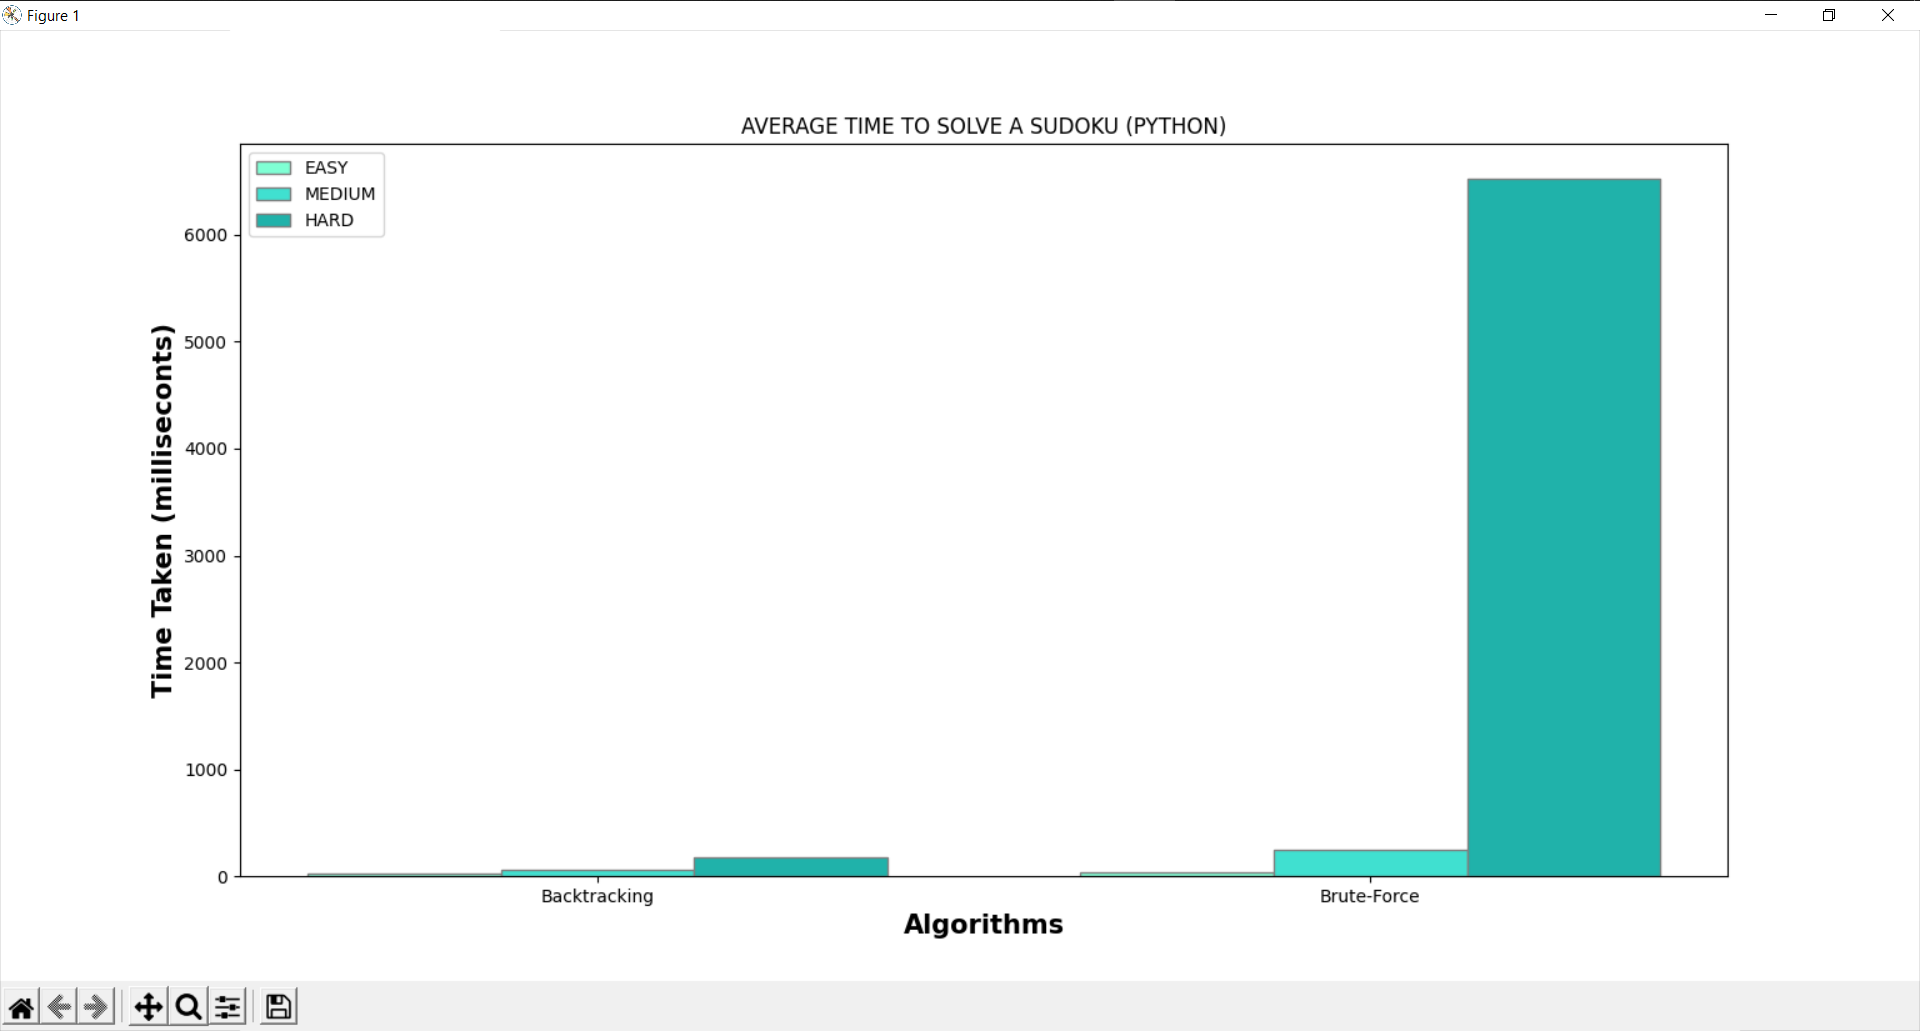
\includegraphics[width=0.9\textwidth]{./week7_img/graph_python.png}
		  \caption{Results: Average time taken to solve a sudoku in Python.}
		  \centering
		  \end{figure}
\end{frame}

\begin{frame}
     \frametitle{Current Status}   
		  \begin{figure}
		  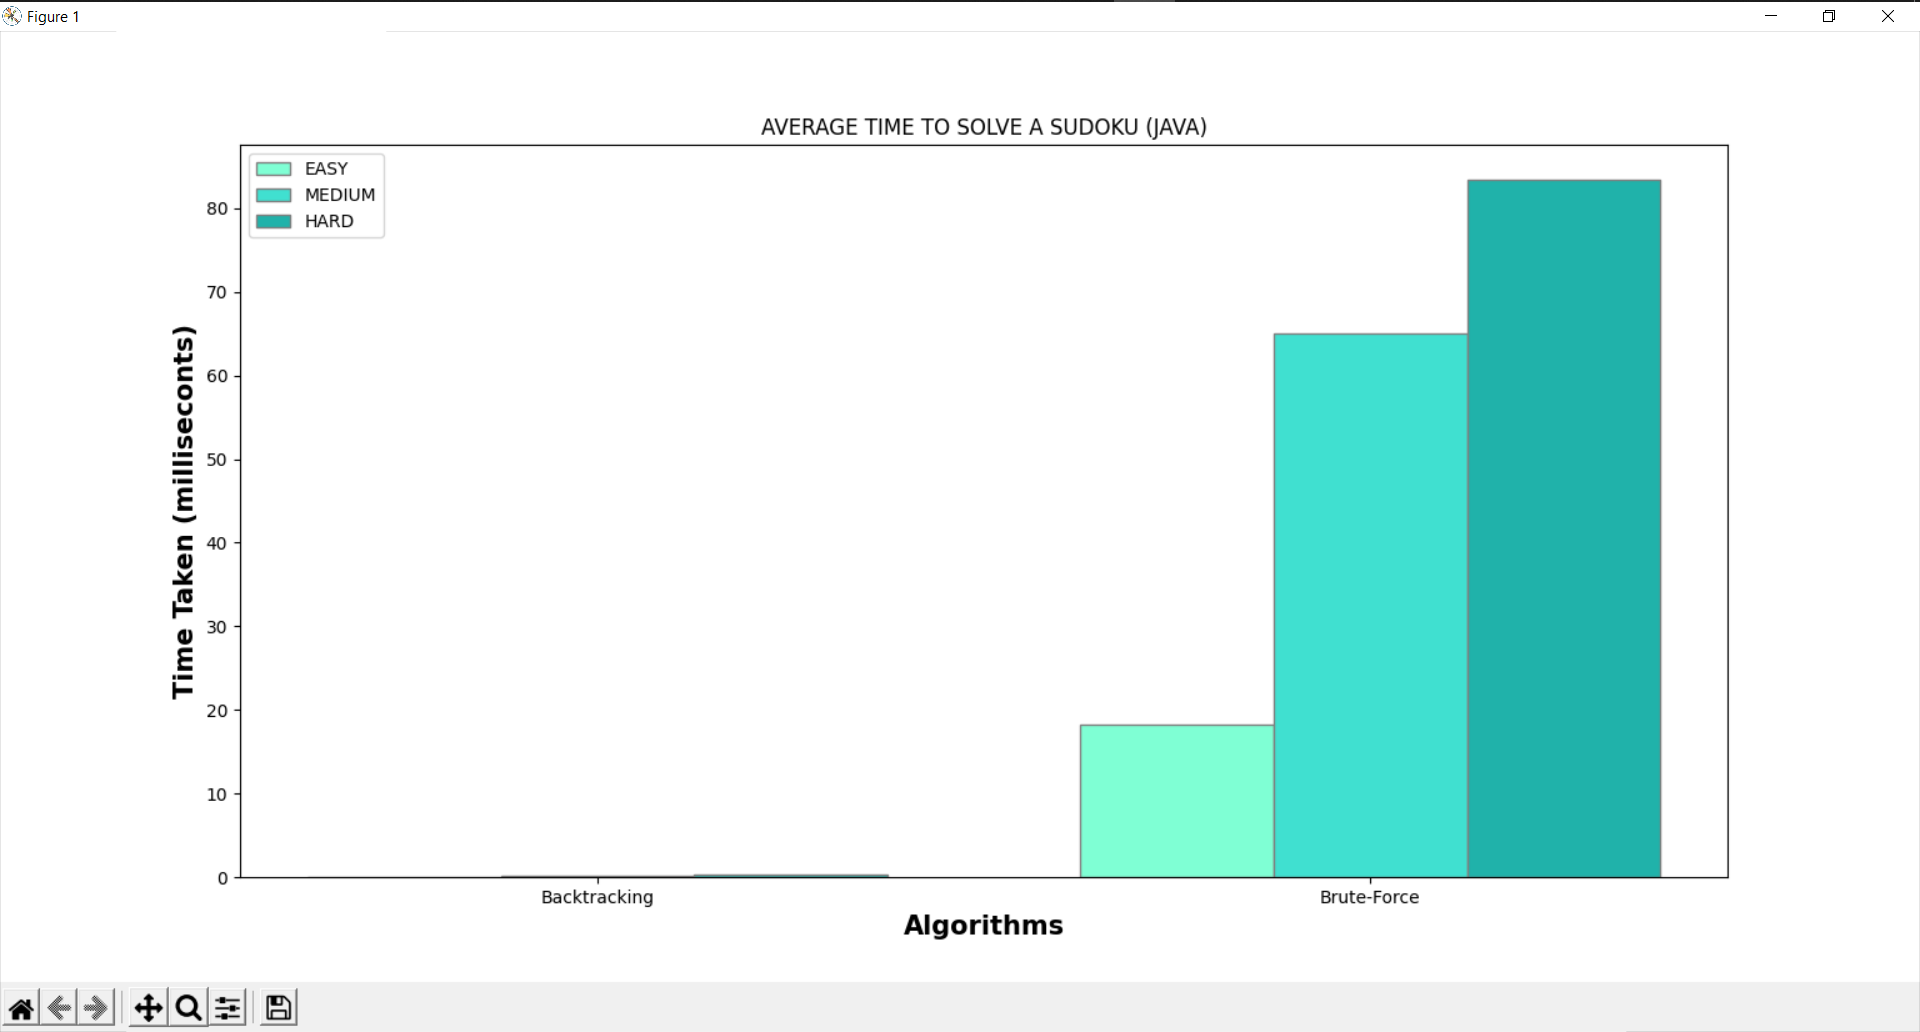
\includegraphics[width=0.9\textwidth]{./week7_img/graph_java.png}
		  \caption{Results: Average time taken to solve a sudoku in Java.}
		  \centering
		  \end{figure}
\end{frame}

\begin{frame}
     \frametitle{Current Status}   
		  \begin{figure}
		  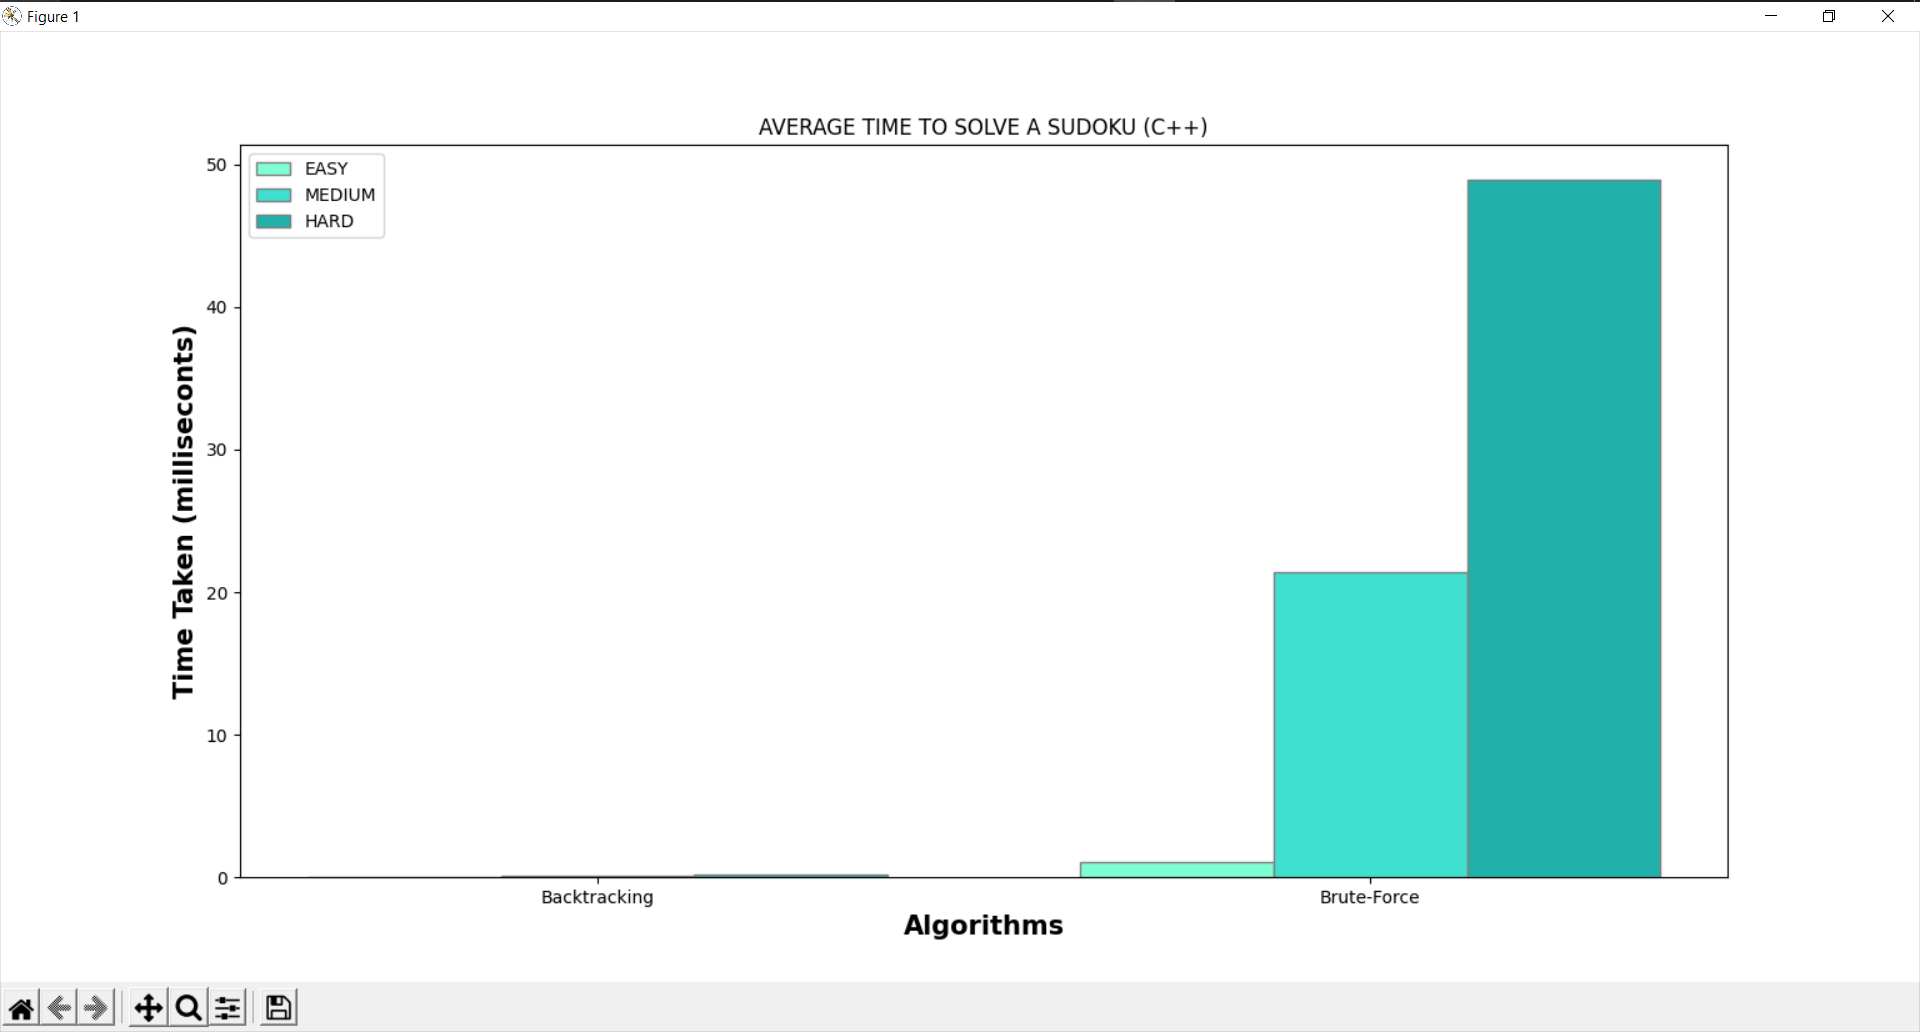
\includegraphics[width=0.9\textwidth]{./week7_img/graph_C++.png}
		  \caption{Results: Average time taken to solve a sudoku in C++.}
		  \centering
		  \end{figure}
\end{frame}


\begin{frame}
	\frametitle{Current Status}
	\begin{itemize}
	      \item Completed image processing of a sudoku puzzle image.
		  \begin{figure}
		  \includegraphics[width=0.9\textwidth]{./week7_img/image_processed.png}
		  \caption{Image processing of a random sudoku puzzle image.}
		  \centering
		  \end{figure}
		  \item Read and learnt concepts of neural networks, machine learning and image processing.
	\end{itemize}
\end{frame}

\begin{frame}
     \frametitle{Toolchain}
     \begin{itemize}
          \item Languages: Python,C++, Java, Haskell, Elixir.
          \item Libaries Used: time module (in Python, C++ and Java) and matplotlib(python)
          \item Open CV 
     \end{itemize}
\end{frame}

\begin{frame}
     \frametitle{Difficulties}
     \begin{itemize}
          \item The backtracking algorithm took some time to implement because we had few challenges implementing the recursive function.
		  \item Understanding Stochastic Simulated Annealing was difficult. The resources for this algorithm were quite less.
	      \item For stochastic and crook's algorithm approach, the sudoku solver does not work for all cases. This requires a little bit of work.
		  \item Explaining each other's ideas to each other took a while.
		  \item Generating 100 sudokues of 3 different difficulty levels was a challenge because it was taling lot of time to generate the puzzle and we had to optimize the code.
		  \item Understanding the concepts of Image Processing and neural networks took us a while.
\end{itemize}
\end{frame}

\begin{frame}
     \frametitle{Learnings}
     \begin{itemize}
     \item Learning about the implementation of different algorithms to solve a Sudoku.
     \item Collaboration and understanding git commands.
	 \item Explaining our code, thought process and ideas to each other.
	 \item Understanding the concepts implemented in Stochastic algorithm using Simulated Annealing.
	 \item Generating data in one language, importing and using the data in another language.
	 \item Learnt about neural networks and its applications.
\end{itemize}         
\end{frame}

\end{document}


